%=========================================================================
% (c) Michal Bidlo, Bohuslav Křena, 2008

\chapter{Virtualization}

\section{Virtualization basics}
In short, virtualization means emulation of hardware within a software platform. Although it may seem that virtualization is the invention of last few years its concept was first brought up in 1960s. It was firstly implemented by IBM to split resources of their massive mainframe machines among multiple virtual machines that could work independently from each other. Therefore they use resources more efficiently.

To further explain basics of virtualization I would like to start by brief explanation of architecture of standard computers. First, we need hardware layer which contains processing unit, storage and other hardware devices, on top of this layer is operating system which abstracts functioning of hardware layer and offers application layer means to communicate with HW layer. Operating system runs as privileged software which means that it is generally able to perform any operation supported by hardware. Its role is to create an interface which simplifies or ignores implementation of components on lower levels of a hierarchy to make using them on application level easier. On the top of an operating system is the application layer which consists of user programs which are less privileged and can generally perform only operations that are permitted to them by operating system.

\begin{figure}[H]
\centering
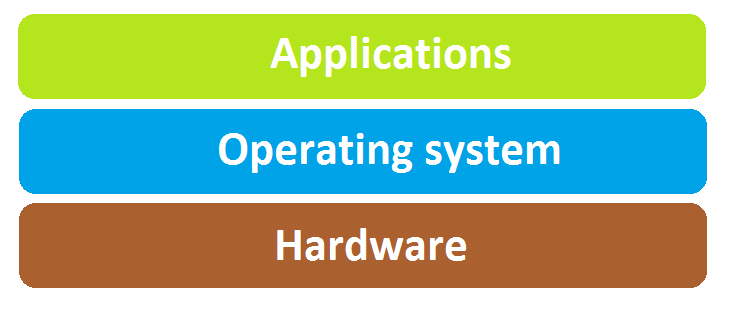
\includegraphics[scale=0.5]{klasika.png}
\caption{Standard architecture}
\end{figure}

Virtualization allows creating multiple entities of operating system and application layers on single HW layer. This is done by inserting additional layer of system software between operating system and lower layers. This virtualization layer is called hypervisor or VMM (virtual machine monitor) and there are two main types of it:
\begin{itemize}
\item Type I hypervisor (or bare-metal/native hypervispor) \label{type_i_hyp} runs directly on host system's hardware with highest level of privilege and has full control over application layer running on top of it. Type I hypervisors have generally better performance than type II hypervisors because they don't have to communicate with hardware layer through operating system thus can utilize full potential it. Some of them need special privileged virtual machine called Domain-0 from which it can be managed and controlled.

\begin{figure}[H]
\centering
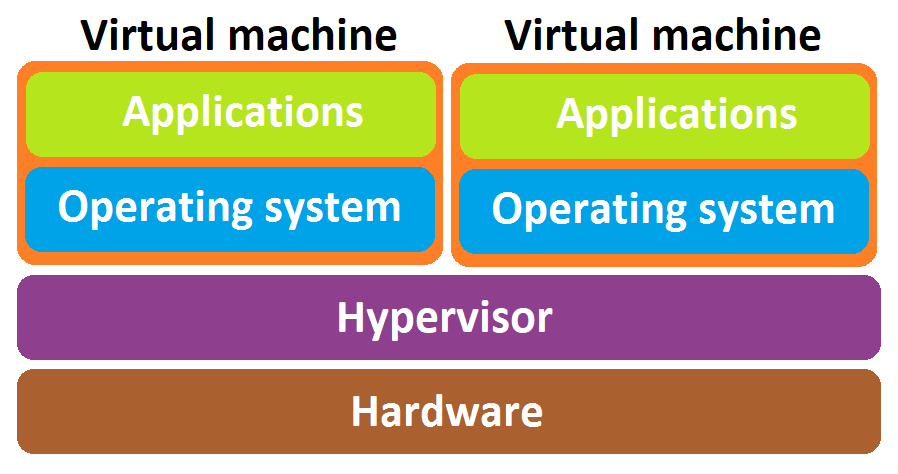
\includegraphics[scale=0.4]{hyp-type-I.png}
\caption{Type I hypervisor}
\end{figure}

\item Type II hypervisor (or hosted hypervisor) \label{type_ii_hyp}: runs on top of the host operating system in an application layer. This means that hypervisor doesn't require specific drivers for I/O operations and allows running the virtual environment within already existing environment. It is less efficient than type I hyperisor because communication between virtual machines and hardware transitions also through operating system but on the same level as hypervisor can run applications directly on host operating system.

\begin{figure}[H]
\centering
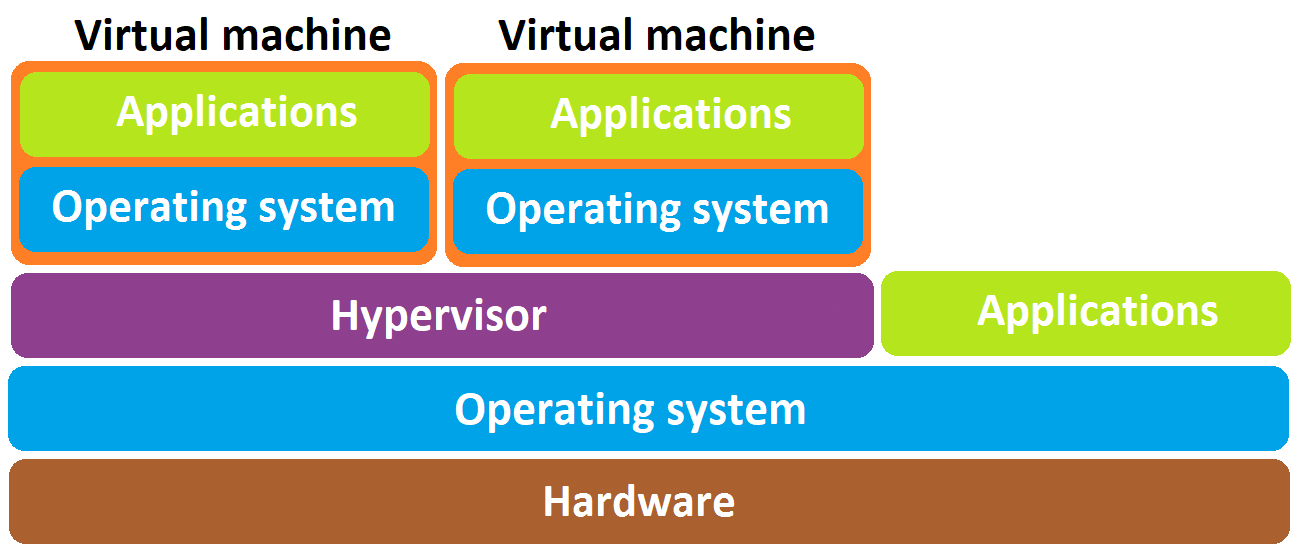
\includegraphics[scale=0.4]{hyp-type-II.png}
\caption{Type II hypervisor}
\end{figure}

\end{itemize}

\section{Advantages of virtualization}
As every other technology, virtualization have some advantages and disadvantages. Lets start with advantages:
\begin{enumerate}
\item Efficiency: Virtualization allows more efficient use of host machine - multiple virtual machines can run different services. Running multiple services on same server can be dangerous for multiple reasons so it is considered a bad practice. Most obvious problem is with hardware overhead, if numerous very resource-demanding services run on single physical machine it can slow it down considerably or even crash it which makes business's services very unreliable. On the other hand, if we run only single service on whole physical host, that service can use for example only 20\% of server machine's resources (this is very common especially noways as hardware is becoming more and more powerful and the average service utilizes only about 10\% to 15\% of all available resources). This way we waste remaining 80\% of resources which, in the long run, unnecessarily raises expenses on managing physical hosts. Rather, we can run various virtual servers on one physical hardware and on each of them run single service.
\item Cost reducing: By concentrating virtual machines on fever hosts we can reduce expenses associated with running large number of physical machines in various ways. We need less physical space for storing hosts, less energy for cooling is needed, less energy is spent on powering the hardware and managing fewer physical devices is also easier and cheaper. Companies with fewer than 1000 employees spend up to 40\% of their IT budget on hardware[], which is the cost that can be greatly reduced by virtualization. Although this benefits more larger companies using plenty of server machines, smaller companies can benefit greatly from virtualization too. Using less energy/space/etc. means that virtualization is also friendlier to environment.
\item Flexibility: Increasing the number of physical workstations or servers is very financially and time consuming process. We need new physical space, order new machines, set them up and so on. With suitable use of virtual machines, the whole process can be easier and faster. There are no more additional hardware costs and administrators can easily setup and manage virtual machines using virtual machine management software. By using templates we can make creating new virtual machines even faster by automatizating of setting up procedures. When some hardware which hosts virtual machines becomes obsolete or it just needs to be out of service for maintenance reasons, we can migrate vms to another physical hardware.
\item Testing: Virtual machines are completely isolated from each other which gives us possibility for testing environments with completely different operating systems and configurations. Even extreme situations are easy to set up or changed. Compared to physical machines, virtual machines can be added and removed very fast. QA teams often have multiple virtual machines with which they speed up testing and therefore development process.
\item Security: All virtual machines are confined entities separated from other software so when one of them gets attacked, gets virus, or for any reason fails, only that one virtual machine fails. While problematic virtual machine is being diagnosed and repaired, another backup virtual machine can take it's place and continue running it's service which greatly reduces down-time and increases reliability of service.
\item \label{live-migration} Isolation: Virtual machines are hardware independent which means that their current state can be captured and reproduced on another physical host in process called migration. This reduces down-time even more because we can run all our services temporarily from another host while former host is being down due to maintenance. There is also a possibility of live migration - i.e. migration without downtime. It is the ability to move running virtual machine between physical hosts with no interruption of service. The virtual machine remains powered on and user applications continue on running while the virtual machine is relocated to a new physical host. In the background, the virtual machine's RAM is copied from the source host to the the destination host. Storage and network connectivity are not altered.
\end{enumerate}

\section{Disadvantages of virtualization}
Disadvantages: 
The disadvantages of virtualization are mostly those that are associated with any transition to a new technology and can be overcame by careful planing and professional implementation.
\begin{enumerate}
\item Overloading: This problem lies in wrong or incomplete estimation of amount of hardware resources needed to handle desired virtual environment. Virtualizaion carries along additional bandwidth in form of hypervisor and other components which is not neglectable. Other extreme is not utilizing full potential of physical host capabilities and wasting resources in long run by using more hosts that are actually needed. Basic rule of thumb is to use around 80\% of physical machines resources.
\item Bandwidth: The volume of data transfered through network might be too much to handle for single network interface card (NIC), this can lead to slower network transfers and therefore offering of services. One of possible ways to solve this is to use host machine with multiple NICs.
\item Need for adjustments: In some cases, adapting a virtualization technology requires rewriting or patching some pieces of software to be compatible with virtual environment.
\item Cost: To run multiple machines on a single host machine, we need it to be sufficiently powerful. This means that additional investments into hardware may be needed. Another investments are into virtualization software and managing virtual machines.
\item Learning curve: Conversion to and managing virtual environment will require IT staff with necessary training. The beginning stages can be painful due to lack of experience with new technology. Many modern virtualization solution vendors offer trainings for their products.
\item Vulnerability: Although virtualization brings certain security benefits it also brings a big risk in form of potential damage cost by lower level layers corruption. In physical environment, if an operating system of one machine gets corrupted than only that one machine is affected. But in virtualized environment if hardware, operating system or hypervisor of a host gets damaged than all virtual machines running on it can potentially become unavailable. This problem can be reduced by regular backups and snapshots which allow easy transfer of virtual machines to a new host.
\item Licensing: Majority of software vendors consider virtual machine to be exactly the same as physical machine so if certain piece of software is needed on multiple virtual machines than we have to pay for a license for each one of them. We can try to solve this by using open-source software. This is becoming less of a problem nowadays because more and more software vendors are adjusting their view on virtualization (for example Windows Server 2016 uses Per Core Licensing which means that each copy of Windows Server will license 2 physical processor cores).
\end{enumerate}

\section{Virtualization architectures}
Virtualization technology is spreading rapidly and today there are several architectures that implement this concept. Here are basic architectures and in chapter 2 we will discuss some of their implementations.
\begin{enumerate}
\item Full virtualization
\item Paravirtualization
\item Operating system virtualization
\item Other types of virtualization
\end{enumerate}

\subsection{Full virtualization} \label{full_virt}
Provides a total virtualization of hardware which means that every virtual entity runs as it is running on a physical hardware completely unaware that its platform is being virtualized. When a virtual machine wants to access hardware it accesses virtual hardware provided by a hypervisor which finally accesses physical hardware. Hypervisor thus acts as the only bridge between virtual machine and physical hardware. This is a reason why the full virtualization is in terms of performance behind non-virtualized machines.
\subsubsection{Software assisted virtualization}
Historically, the first full virtualization solution introduced in 1969. With this approach, every part of a physical hardware is virtuallized which has advantage in fact that every operating system or application can be run completely without modifications. On the other hand every operation made by operating system of virtual machine needs to be simulated and checked if it doesn't conflict with any other virtual machine or hypervisor which makes this process very resource-expensive.

\begin{figure}[H]
\centering
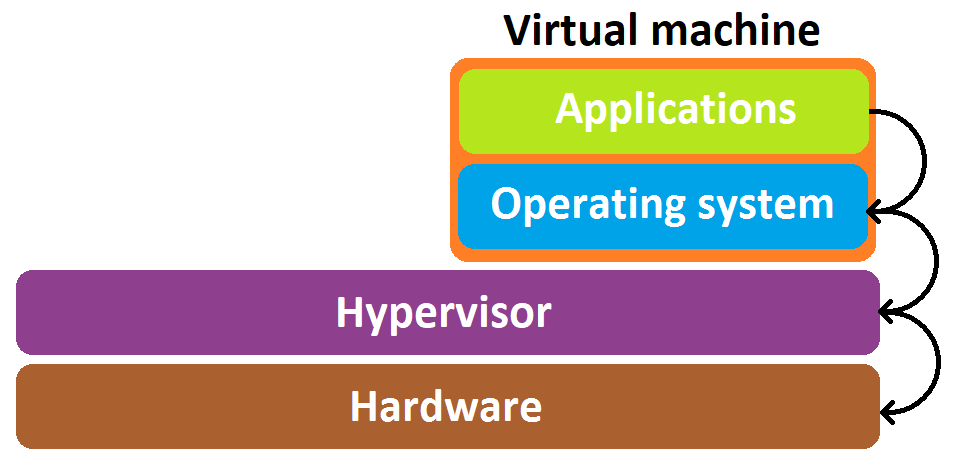
\includegraphics[scale=0.4]{sw-assist.png}
\caption{Software assisted virtualization}
\end{figure}

\subsubsection{Hardware assisted virtualization}
Introduced by IBM in 1972. This approach reduces the problem of massive overhead in software assisted virtualization by extending functionality of hardware (mainly CPU) by new instructions allowing virtual machines to directly access physical hardware without expensive mediators. Normally x86 operating systems need to have a direct access to hardware resources, software-based virtualization solves this problem by virtualizing entire hardware layer but for price of wasting a big chunk of hardware resources. In hardware assisted virtualization is this overhead noticeably reduced because processor no longer needs to be emulated and can directly interact with application layer. Another advantage is that it will work 'right of the box' meaning that we don't need to upgrade or change anything, all we need to do is to use processor supporting hardware-based virtualization technology. Main representatives of this method are Intel VT and AMD-V.

\begin{figure}[H]
\centering
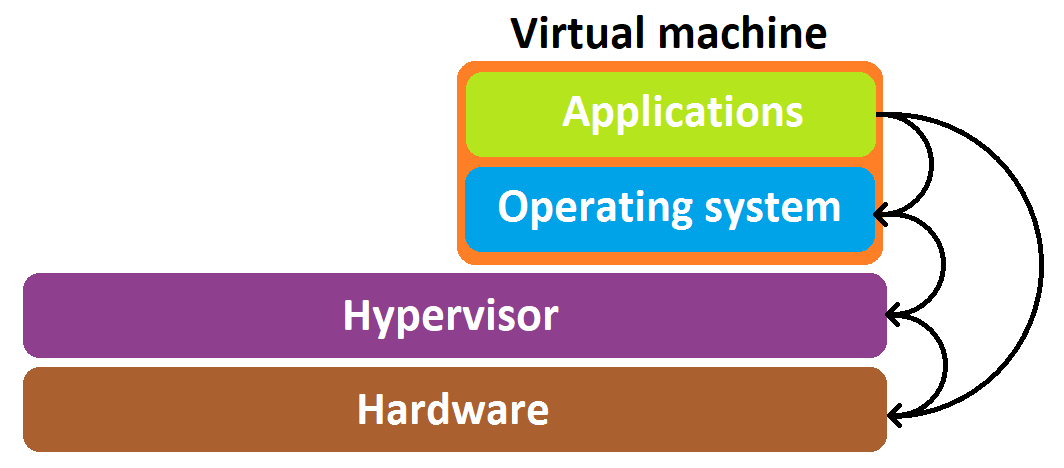
\includegraphics[scale=0.4]{hw-assist.png}
\caption{Hardware assisted virtualization}
\end{figure}

\subsection{Paravirtualization} \label{paravirtualization}
Introduced in 1972 by IBM, this technique was implemented to increase performance of virtualized environment closer to non-virtualized. To use paravirtualization, kernel of the operating system needs to be modified, mainly it needs to have replaced all privileged operation running only in ring 0 by so called 'hypercalls'. Hypercalls allow guest operating system to send system calls directly to the hypervisor without the need of hardware simulation. Virtual machine can therefore access some part of the hardware straight without going through virtualized hardware on the top of hypervisor which greatly increases performance of some operations. This only works for some parts of the hardware, for other parts, virtual machine still needs to use virtualized hardware. Paravirtualized virtual machine is 'aware' of the fact that it is being virtualized which gives it ability to use hypercalls. On the other hand, as mentioned above, in order to use this technique, operating system needs to be altered in a non-trivial way which typically limits its use to a Linux based operating systems because they allow such source code modifications.
Paravirtualization was popularized by Xen hypervisor, today, most virtualization solutions use it as a norm (for example Red Hat Xen, VMware's family and others).

\subsection{Operating system virtualization} \label{os_virt}
Also known as shared kernel virtualization, introduces 'light-weight' virtualization. To understand this concept, first we need to have at least very basic understanding of what are kernel and root file system and what are their roles. Kernel is central part of the operating system, which mediates communication between other parts of operating system and physical hardware. Root file system contains all the files, libraries and practically all utilities necessary for operating system to work properly. In shared kernel virtualization every virtual machine has its own root file system but uses host operating system's kernel which they share among each other. Kernel has the ability to dynamically switch the current root file system to a different one without the need to reboot the whole system (technique also known as 'chroot'). In this case, virtual machines are referred to as 'containers' due to the fact that they are not completely separated but share host machine's kernel. Shared kernel means very little overhead compared to other virtualization concepts and thus higher performance rate. Despite its light-weight nature, this concept also supports advanced features such as isolating memory space, regulating memory, network, CPU and I/O usage, some implementations even allow live migration. Biggest advantage of container-virtualization is superior efficiency and very little overhead compared to other types of virtualization because it doesn't have to emulate all the hardware. Interactions between software and hardware are handled by operating system's kernel inside container. Major disadvantage of this technique is that container's operating system must be compatible with kernel on which it runs (container operating system must be designed for type and version of kernel that is being shared). Further, container environments cannot execute some top-level actions, mount or dismount file systems and so on whereas fully virtualized solution gives us fully independent environment in which isn't user restricted in any way.
Well known solutions are Linux VServer, Jail for FreeBSD, Zone for Solaris, Virtuozzo for Windows, Rosetta for Mac OS and others.

\begin{figure}[H]
\centering
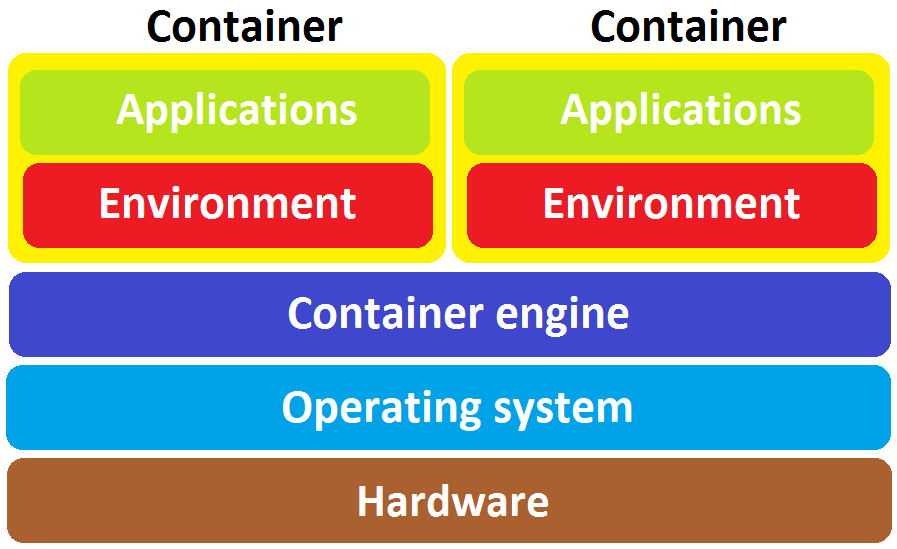
\includegraphics[scale=0.4]{container.png}
\caption{Operating system virtualization}
\end{figure}


\subsection{Other types of virtualization}
\subsubsection{Network virtualization}
Main idea is to create multiple virtual sub-networks (channels) that run on single physical network and are independent from one another. Each one of virtual networks can have different bandwidth related, security or other restrictions and we can regulate traffic on each channel independently.  Monitoring individual networks with their own purposes and settings is also easier and faster, it increases reliability and durability of network too as if one of virtual networks is for whatever reason overloaded or down other networks are not affected. Most modern hypervisors implement virtual networking in some form. Network virtualization can be further divided into two sub-categories:
\begin{enumerate}
\item Internal: can be used for communication between software and virtual machines or to mimic network to external devices. Internal network uses virtual network devices that act as physical devices and enables single system to appear as a network.
\item External: used in Virtual local area networks (VLAN) and Virtual private networks (VPN).
\end{enumerate}

\subsubsection{Application virtualization} \label{app_virt}
This technique separates the application layer from the underlying operating system layer which means that application runs in 'encapsulated' state independently from operating system. Application is put into a capsule which contains copies of all shared resources that application would need to run as well as all DLLs (dynamically linked libraries), drivers, registry entries and so on. 

In practical terms it means:
\begin{enumerate}
\item Application created for certain operating system can run on a different one, for example native Windows applications can be run under Linux distribution or vice-versa.
\item We can isolate suspicious or malicious software and inspect it without the danger of infecting the whole system.
\item Simultaneously running applications that would otherwise conflict each other.
\item Easy deployment applications.
\end{enumerate}
Some well known examples are Wine which is used to run Microsoft Windows applications on Linux, ThinApp from VMware, Xenocode from Code System Corporations and others.

\begin{figure}[H]
\centering
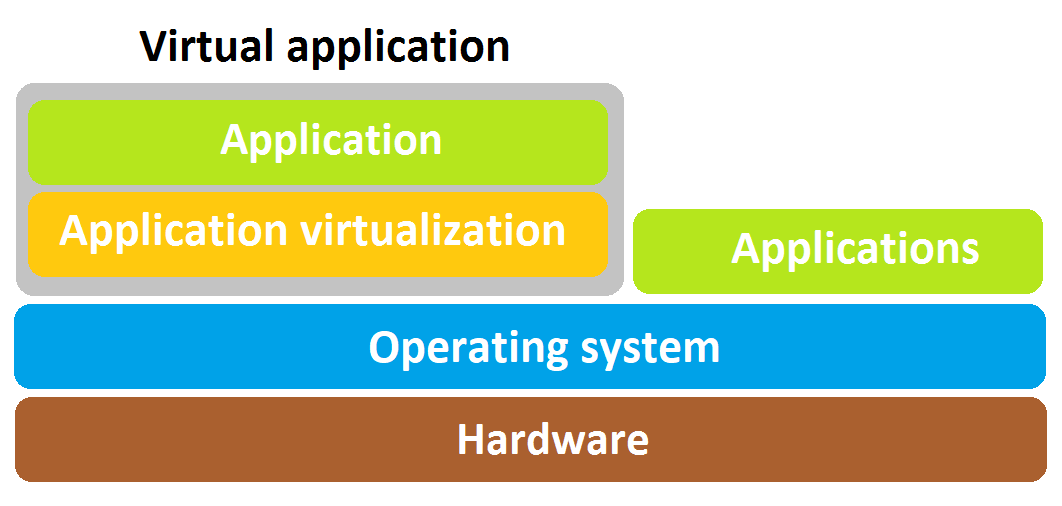
\includegraphics[scale=0.4]{app-virt.png}
\caption{Application virtualization}
\end{figure}


\subsubsection{Desktop virtualization} \label{desktop_virt}
Similarly as application virtualization it separates desktop environment from underlying physical computer. Desktop virtualization functions on a client-server model. Client desktop environments run on virtual machines stored on servers and can access them via client device which can be standard PC, tablet, thin client which is specialized device capable of displaying virtual desktop environment or others. This technique is growing on popularity mainly because of cloud computing. It allows us to access desktop from any device or location (in practical terms it means that we can work in same environment from anywhere without the need to bring 'work computer'). By using desktop virtalization we can use cheaper client desktop devices because far less processing power is required. Of course, businesses need to first invest into server hardware so it is capable of storing and streaming desired quantities of desktop environments but will save money in a long run by cheaper user devices. Desktop environments are stored on central server so they can be also centrally managed and controlled which increases security of whole system. Disadvantage is that streaming desktop environments to plenty of end users is very demanding on network infrastructure. Desktop virtualization is mostly used by companies with a lot of off-shore employees.

\subsubsection{Storage virtualization}
Multiple separated hardware storage devices (that can be on different physical locations) abstracted into single pool of virtualized storage space that act as a single storage device locally connected to the computer. Storage virtualization is used to ignore differences between individual storage devices and simplify using them. It is often used for back-ups and archives and can be implemented with software or hybrid software-hardware solutions. Common examples are:
\begin{enumerate}
\item DAS: (Direct Attached Storage) is a disk subsystem that is directly connected to a host rather than going through a switched network, thereby giving the host exclusive access to the disks.
\item NAS: (Network-attached storage) is server dedicated to managing storage space. NAS devices have to be part of LAN and they can be added or removed dynamically meaning that after adding/removing device whole system doesn't need to be restarted but it continues functioning as if nothing have happened.
\item SAN: (Storage area network) is basically a sub-network containing only storage devices. Storage space managed by SAN can be accessed by any server in LAN or WAN. When new storage devices is added it is immediately available to any server in network. In practical sense SAN enables anyone within network have access to network's whole storage space.
\end{enumerate}


\chapter{Virtualization software}
In this chapter we will go through the following virtualization implementations.
\begin{enumerate}
\item Xen Project
\item KVM
\item VirtualBox
\item UML
\item Docker Container
\item Wine
\end{enumerate}

\section{Xen Project} \label{xen}
Is well known type I hypervisor which means it runs directly on the host hardware. Xen Project is widely used as base for a number of open-source and commercial applications providing server and desktop virtualization, infrastructure as a service (IaaS), security applications, embedded and hardware appliances and so on. Worlds biggest clouds today also run on Xen Project hypervisor base. All operating systems based on recent Linux kernel are capable of running Xen project and have packages containing hypervisor and basic tools.

Xen is managed by a special privileged virtual machine called Domain-0 or Dom0, privileged means that it has device drivers and direct access to physical hardware. Domain-0 is a specially modified Linux kernel which is started by Xen hypervisor during initial stage of system start-up(!). Its role is to manage and control every other unprivileged virtual machine (also called Domain-Us or DomU) that is running on the hypervisor. Domain-0 exposes control interface to the user and Xen project hypervisor cannot run without it. Through user interface in form of toolstack (or control stack) user can create, delete or configure virtual machines, toolstack can by driven by command line console, graphical interface or cloud orchestration stack (for example OpenStack or CloudStack).

Originally Xen only supported paravirtualization (see \ref{paravirtualization}). Support for Domain-U running in paravirtualized state is now included within upstream Linux kernel but support of Domain-0 is not which means that it is easier to use Linux machine as a guest than as a host. Nowadays Xen supports the new virtualization processor extension added to the x86 architecture(!), this is known as Xen Hardware Virtual Machine (HVM). HVM allows unmodified guest operating system to be virtualized on Xen hypervisor(!) but it requires a special processors that support hardware virtualizaton extensions (Intel VT, AMD-V). These extensions allow for many of the privileged kernel instructions to be handled directly by hardware using 'trap-and-emulate' technique (previously in paravirtualization converted to hypercalls).

Trap-and-emulate: Operating systems running on top of the hypervisor are run as user-level processes. They are not running at the same level of privilege as a Linux operating system that is running on bare metal. But if the operating system code is unchanged, it doesn't know that it does not have the privilege for doing certain things that it would do normally on bare metal hardware. In other words, when the operating system executes some privileged instructions, meaning they have to be in a privileged mode or kernel mode to run on bare metal in order to execute those instructions, those instructions will create a trap that goes into the hypervisor and the hypervisor will then emulate the intended functionality of the operating system. This is what is called the trap and emulate strategy. Problem in some architectures is that some privilege instructions may fail silently which means that you would think that the instruction actually succeeded, but it did not, and you may never know about it.

\begin{figure}[H]
\centering
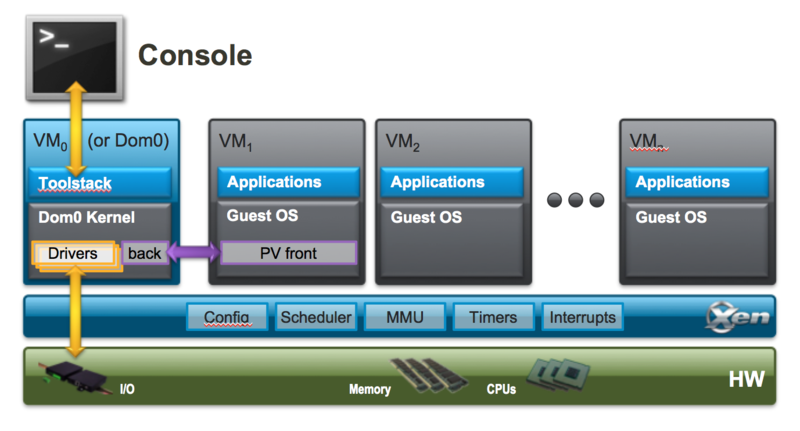
\includegraphics[scale=1]{xen-diagram.png}
\caption{Xen architecture}
\end{figure}

Here are key features of Xen project hypervisor:
\begin{enumerate}
\item Minimal footprint: around 1 MB. Xen uses micro-kernel design which minimalizes memory footprint and interface to the guest and is also more robust and secure than other types of hypervisors.
\item Driver isolation: hypervisor allows for the main device driver to run inside of a virtual machine. This is useful because if driver crashes it does not affect any other part of a system and virtual machine in which it runs can be rebooted and the driver restarted.
\item Support many operating systems: although most installations use Linux as the domain-0 many other operating systems can by used such as NetBSD, OpenSolaris and others.
\end{enumerate}


\section{KVM} \label{kvm}
KVM - Kernel-based Virtual Machine little less known virtualization solution then Xen Project. It has host and guest support in an upstream Linux kernel released in early 2007. KVM is kernel module which when loaded turns host kernel into type I hypervisor. Running it requires Intel VT or AMD-V extensions enabled on a host system. By converting host machine kernel into hypervisor, KVM can take advantage of already implemented components instead of implementing them from the scratch. For example it uses memory manager, scheduler, I/O stack, device drivers, security manager, network manager and others. In comparison to the Xen architecture which requires maintenance of both Xen hypervisor and Domain-0, KVM is loadable kernel module and is easier to patch and upgrade. From host's perspective, every virtual machine is standard Linux process and is treated as such.

Features:
\begin{enumerate}
\item Security: to improve security of virtual machines even further, KVM uses these approaches:
\begin{enumerate}
\item Security-enhanced Linux (SELinux) which establishes security boundaries around virtual machines.
\item Secure virtualization (sVirt) which boosts SELinux's capabilities and allow Mandatory Access Control (MAC) security to be applied.
\end{enumerate}
\item Live migration: KVM supports live migration (see \ref{live-migration}) of virtual machines.
\item Scheduling and resource control: every virtual machine is seen as a standard process which means that Linux scheduler allow full control over resources allocated by it and guarantees quality of service. KVM offers completely fair scheduler, control groups, network name spaces and real-time extensions.
\item Storage: KVM supports shared file system which means that virtual machines can be shared by multiple hosts. Disk images support thin provisioning. Thin provisioning means that memory is allocated for virtual machine up to provisioned amount only when it needs it (Xen Project doesn't support thin provisioning, when virtual machine is provisioned for example 2 GB of RAM, after it starts, 2 GM of RAM are immediately allocated and can't be used elsewhere). This can lead to 'memory overcommit', state where more memory is assigned to virtual machines than is actually available on the system. KVM deals with memory overcommit in various ways:
\begin{enumerate}
\item Host can choose memory pages and write them to the disk. This leads to reducing performance because when virtual machine wants to access memory, host needs to read it from the disk which is significantly slower than RAM memory.
\item With VirtIO drivers, host can request virtual machines to shrink their cache memory in order to free as much space as needed. This is called 'ballooning' and requires cooperation among host and guests.
\item KSM (Kernel Samepage Merging) is a process of merging identical memory pages from multiple virtual machines into a single read-only memory chunk while removing all duplicates of it. If any guest needs to write into one of merged pages, host creates writable copy which guest can modify.
\end{enumerate}
\item Lower latency: kernel divides processes with long computing times into smaller pieces which are scheduled and processes accordingly.
\end{enumerate}


\section{VirtualBox} \label{virtualbox}
VirtualBox is a type II hypervisor currently being developed by Oracle Corporation. Oracle VM VirtualBox runs on Microsoft Windows, Mac OS X, Linux and Oracle Solaris systems and supports wide range of guest operating systems. With thousands of downloads each day it is the most popular cross-platform open-source virtualization solution.

Here are some of VirtualBox's main features:
\begin{enumerate}
\item Portability: VirtualBox has to run on an host operating system but its functionality is to a very large degree identical on all of them, same files and image formats are used. This allow us to create a virtual machine on one host and run it on another host with different operating system. Virtual machines can be imported and exported using an Open Virtualization Format (OVP) with which we can import virtual machines created with different virtualization software.
\item No hardware virtualization needed: VirtualBox doesn't require a processor support like Intel VT or AMD-V so it can be run even on older hardware not possessing those features.
\item Guest additions: guest additions are software packages that can be installed inside of virtual machines to improve their performance or improve their integration with host system. They consist of device drivers and system applications, for example on of guest additions is 'Shared folders addition' which provides an easy way to exchange files between host and guest. We can create a folder on host system and share it to the guest.
\item Hardware support:
\begin{enumerate}
\item Guest multiprocessing: VirtualBox can present up to 32 virtual CPUs to every virtual machine regardless of how many CPUs are present in host system.
\item USB device support: virtual USB controller allows to connect USB device to virtual machine without a need to install device-specific drivers to the host machine.
\item ACPI support: Advanced Configuration and Power Interface is an open standard that operating systems can use to configure hardware components and to perform power management and status monitoring.
\item Built-in iSCSI support: this allows us to connect from virtual machine directly to the iSCSI storage server without going through host system which
highly reduces overhead.
\item PXE support: Preboot eXecution Environment (PXE) in short is a way to boot operating system from a server on a virtual machine. Advantages are obvious, we don't need to have a operating system on a hard drive connected to the virtual machine, we just need to connect to server and boot it from there.
\end{enumerate}
\item Snapshots: we can create snapshots of the current state of a virtual machine and store it. When needed we can reverse current state of VM and load configuration from any snapshot. This way we can periodically save backups for quick recovery in case of emergency.
\item Grouping: multiple virtual machines can be collected into a group. We can than perform same operations over the group as we can over individual virtual machines (for example start, pause, shutdown, close, ...). By using groups we can manage multiple virtual machines with same configuration, purpose, etc at the same time as well as we can still manage individual VMs that are part of a group. One virtual machine can be inside multiple groups and groups can be nested into hierarchy.
\item Remote machine display: VRDE - VirtualBox Remote Desktop Extension allows for a high-performance remote access to any running virtual machine.
\end{enumerate}


\section{UML}
User Mode Linux (UML) allows us to run Linux kernels as user mode processes under a host Linux kernel thus allowing us to run multiple independent virtual machines. Main difference between UML and other virtualization technologies is that UML is more of a virtual OS than virtual machine. Other solutions like VMWare are real virtual machines in that they emulate physical hardware and any operating system that runs on physical platform can also run on emulated one. Advantage of this solution is that guest OS is host OS-independent, meaning that any OS able to run on hardware is able to run on top of VMWare. On the other hand, UML is basically just Linux kernel modified to run in user space, UML guest can run only on Linux platform which is serious limitation but being more of virtual OS has other advantages. Solutions such as Xen, BSD jail or Solaris zones are integrated into host operating system but UML runs as a process. This has some performance costs but gives UML host OS version independence. UML has many real-world uses but it's most popular use-case is kernel development and debugging as it was its original purpose, for that can be used normal process-level tools like gdb, gporf (profiling) or gcov (coverage testing). Another popular uses are driver development, safe kernel testing and education due its simpler nature than other solutions.


\section{Docker Container} \label{docker}
Docker container is a operating system level technology established  and promoted by Docker Inc.

Docker uses a technology called namespaces. When we run a container, Docker creates a set of namespaces for it. These namespaces provide a layer of isolation. Each aspect of a container runs in a separate namespace and its access is limited to that namespace.
On Linux, Docker Engine uses these namespaces:
\begin{enumerate}
\item pid: process isolation
\item net: managing network interfaces
\item ipc: managing access to IPC resources
\item mnt: managing file system mount points
\item uts: isolating kernel and version identifiers
\end{enumerate}

Docker container is operated by command-line tool called the Docker client which can run on the container host or through a remote interface connected to the container host. The main task of a Docker client is to pull images of containers from registry. Registry can be public or private and it is a repository of sources for 'ready to run' virtual workloads. Main public registry is Docker Hub which is operated by Docker Inc. but nowadays there are plenty of others. We can pull a container image using Docker daemon and from that image we can build working model for that container. A container is launched by running an image. An image is an executable package that includes everything needed to run an application: the code, a runtime libraries, environment variables, and configuration files. Images that are mostly the same, except for the last few steps, can reduce disk usage by sharing parent layers. A container is a runtime instance of an image - what the image becomes in memory when executed (that is, an image with state, or a user process). Image can also include directives for daemon to preload the container with other components prior to running or directives for the local command line after the local container image is build. The model of images and registries created standardized ways to build, load and manage containerized applications. Docker has been very successful in building a large open-source community which has contributed to the rising number of images in public and private repositories which attracts even more developers and enlarges open-source community. Docker image is defined by text-based Dockerfile which specifies a vase operating system image to start from, commands to prepare/build the image and commands to call when image is 'run'. (Docker runs multiple containerized workloads on the same OS. By using containers, only the programs and their immediate dependencies are hosted by containers, with critical resources provided by the underlying operating system.  This means that containerized systems can load applications faster and consume less resources.). Docker is available on many different operatin systems including most modern Linux distributions, Mac OSX and Windows.

OCI: The Open Container Initiative (OCI) is a lightweight, open governance structure (project), formed under the auspices of the Linux Foundation, for the express purpose of creating open industry standards around container formats and runtime. The OCI was launched on June 22nd 2015 by Docker, CoreOS and other leaders in the container industry [citovane]. The OCI currently contains two specifications: the Runtime Specification (runtime-spec) and the Image Specification (image-spec). The Runtime Specification outlines how to run a "file system bundle" that is unpacked on disk. [tiez]

Docker Engine is a client-server application with these major components:
\begin{enumerate}
\item A server which is a type of long-running program called a daemon process
\item A REST API which specifies interfaces that programs can use to talk to the daemon
\item A command line interface (CLI) client
\end{enumerate}
Docker uses a client-server architecture. The Docker client talks to the Docker daemon, which does the heavy lifting of building, running, and distributing Docker containers. The Docker client and daemon can run on the same system, or you can connect a Docker client to a remote Docker daemon. The Docker client and daemon communicate using a REST API.
A Docker registry stores Docker images. Docker Hub and Docker Cloud are public registries and Docker is configured to look for images on Docker Hub by default. We can run our own private register. We can also buy or sell Docker images or distribute them for free in Docker store.


\section{Wine}
Wine - Wine Is Not an Emulator acronym means that Wine is not a virtual machine, it does not emulate physical hardware and we are not supposed to install Windows or any Windows driver on top of it. Different software programs are designed for different operating systems and are generally not compatible with other operating systems, for example Windows programs can't run on Linux system because they use kernel calls that Linux system doesn't understand thus cannot interpret them, this is the main motivation for Wine. Wine is an implementation of Windows API and can be used as a library to port Windows applications to Unix, basically acting as a bridge between the two. It is a compatibility layer, every time a Windows program tries to perform an action that Linux doesn't recognize, Wine will translate it into one that it does. Wine can also recompile Windows program source code into format understandable for Linux. Even in recompiled form, Wine is still needed to run the program but there are many performance and other advantages to this process. Wine is an open source project.

Features:
Wine is constantly growing in the features it supports, here are some of them:
\begin{enumerate}
\item Support for running, Win64, Win32, Win16 and Dos programs.
\item Optional use of external vendor DLLs.
\item MacOS and Android graphics support.
\item DirectX for games.
\item Support for alternative input devices such as graphics tablets
\item Winsock TCP/IP networking support.
\item Advances Unicode and foreign language support.
\item Fill featured Wine debugger and configuratable trace logging messages for easier troubleshooting.
\end{enumerate}

Executables:
Wines main task is to run Windows executables, here are supported types:
\begin{enumerate}
\item DOS executable: very old programs for MS-DOS.
\item Windows NE executable: (NE - New Executable) They were the native processes run by Windows 2.x and 3.x.
\item Windows PE executable: (PE - Portable Executable) Introduced by Windows 95 and became the standard format for all later Windows versions. Portable Executable means that format of the executable is independent of the CPU, even if the code IS dependent of the CPU.
\item Winelib executable: applications written by using the Windows API but compiled as a Unix executable.
\end{enumerate}

Wine architecture is close to the Windows NT architecture but several subsystems are not implemented yet.


\chapter{Products for virtualization}

Even though virtualization technology was introduced more than 20 years ago it experienced a big boom only in past few years. There are now many companies developing some sort of virtualization technology and offering different products. This is great for customers which can choose from wide variety of virtualization tools depending on type/price/scale and so on. Every year more and more companies decide to virtualize their servers for various reasons. In this chapter we will look at biggest or fastest growing virtualization companies today and present some of their products

\begin{enumerate}
\item VMware
\item Citrix
\item Oracle
\item Microsoft
\item Red Hat
\end{enumerate}

\section{VMware}

\subsection{VMware Workstation}
Is basically industry standard for desktop virtualization - it is a hosted hypervisor. Workstation runs on Windows or Linux and can also run virtual machines with Windows or Linux operating system. Initially launched in 1999 is one of the longest running modern day virtualization applications. VMware Workstation Pro can save the state of a virtual machine as a snapshot which can later be restored, effectively returning the virtual machine to the saved state. It can also group multiple virtual machines into an inventory folder with which we can control (power on/off) all the virtual machines inside it at once.
Key features:
\begin{enumerate}
\item High-performance 3d graphics: Workstation supports DirectX 10 and OpenGL 3.3 to run the most demanding 3D applications with near-native performance in Windovs virtual machines.
\item Massive virtual machines: with Workstation we can create virtual machines up to 16 CPUs, 8 TB virtual disks and 64 GB of memory to run high-performance demanding desktop and server applications in virtualized environments. To improve graphics performance we can allocate  up to 2 GB of available host video memory.
\item High resolution display support: Workstation supports high-resolution display for desktops and also multiple displays.
\item Restricted access to virtual machines: virtual machine can be encrypted and protected by password.
\item Cross compatibility: we can create virtual machines that can run across the VMware product portfolio or even import VMs from another vendors. Virtual machines are transfered in Open Virtualization Format (OVF). OVF specifications provides a means of describing the properties of a virtual system. It is XML based and is used to describe a single virtual machine or a virtual appliance.
\end{enumerate}

\subsection{Workstation Player}
Workstation Player is 'lighter' version of Workstation. It runs on same core as Workstation Pro and vSphere (VMware's cloud computing virtualization platform) but delivers less features. On the other hand it is free of charge for personal non-commercial use. Workstation Player can still create and run virtual machines, but its functionality is limited:
\begin{enumerate}
\item It can run only one virtual machine at a time instead of multiple virtual machines simultaneously.
\item It cannot create or manage encrypted VMs.
\end{enumerate}
Workstation Player is great for 'feeling up' virtualization before investing into full blown solutions or for simple personal use.

\subsection{VMware vSphere}
Serves as a complete platform for implementing and managing virtual machine infrastructure on large scale. vSphere consists of two core components: ESXi and vCenter Server.
\begin{enumerate}
\item ESXi is a bare-metal (type I) hypervisor. It has small footprint (150 MB) which minimizes security threats to the hypervisor. It can support up to 128 virtual CPUs, 6 TB of RAM and 120 devices and offers built-in UI based on HTML5 standards, vSphere command line interface and REST-based APIs. Thin architecture enables it to install in 10 minutes and boot 2 to 3 minutes.
\item vCenter Server: provides a centralized platform for managing VMware vSphere enironment, allowing automation and delivery of virtual infrastructure. From single vCenter instance can be managed up to 1000 hosts and 10000 virtual machines, these numbers can be scaled by using Linked Mode for managing up to 30000 virtual machines across 10 vCenter Server instances and vSphere HA for even more hosts and VMS. Linked Mode replicates roles, permissions and licenses across infrastructure so we can log in and view inventories of all vCenter Servers. We can use 3rd-party plug-ins created by VMware partners. With open Web Client Plug-in SDK vCenter Server has largest partner ecosystem in industry which means that we can implement back-up, data protection, server, network and security management directly from vCenter. Web Client Plug-in Certification Program ensures better end-user experience. Certified Plug-ins deliver optimal performance, better security model and so on. We can also back up vCenter Appliances to a file via industry standard protocols. In case of need we can point a fresh appliance to a backup location and files will be downloaded to the new vCenter Server Appliance.
\end{enumerate}

\subsection{VMware ThinApp}
VMware ThinApp is VMware's solution for application virtualization (see \ref{app_virt}). ThinApp uses a build process to package application files and registry settings into a single application container that can be executed on a variety of operating systems without installation. Applications can be executed from a user's desktop, a network path, or removable media. Applications run entirely in user mode under the security context of the currently logged in user. To virtualize an application ThinApp uses a Capture and Build process which consists of two components:
\begin{enumerate}
\item Setup Capture: The Setup Capture wizard guides the process of capturing the application and applying administrator-supplied configurations specific to the package. Setup Capture takes a prescan snapshot, allows the administrator to install and configure the application, and takes a postscan snapshot. The difference between the prescan and postscan snapshots, which represents the application, is placed in the project directory.
\item The process by which the project directories and configuration settings are compressed and embedded into the package.
\end{enumerate}

\section{Citrix}
Citrix Systems, Inc. is an American multinational software company that provides server, application and desktop virtualization, networking, software as a service (SaaS), and cloud computing technologies. The company began by developing remote access products for Microsoft operating systems. It licensed source code from Microsoft and has been in partnership with the company throughout its history. Citrix came to prominence in the 1990s as a leader in thin client technology, purpose built for accessing remote servers. The company had its first initial public offering in 1995 and, with few competitors, experienced large revenue increases between 1995 and 1999. Between 2005 and 2012, Citrix acquired more than a dozen other companies, allowing it to expand into server and desktop virtualization, as well as others.

\subsection{XenServer}
XenServer is the complete server virtualization platform from Citrix. The XenServer package contains everything needed to create and manage a deployment of virtual x86 computers running on Xen (see \ref{xen}), the open-source paravirtualizing hypervisor with near-native performance. XenServer is optimized for both Windows and Linux virtual servers. XenServer runs directly on server hardware without requiring an underlying operating system (type I hypervisor - see \ref{type_i_hyp}). There are two methods by which to administer XenServer: XenCenter and the XenServer Command-Line Interface (CLI). XenCenter is a graphical, Windows-based user interface. XenCenter allows you to manage XenServer hosts, pools and shared storage, and to deploy, manage and monitor VMs from your Windows desktop machine. Key features include creating virtual machine templates from snapshots, XenMotion which allows us to live migrate VMs between hosts. XenServer 7 provides support for high-performance enhanced 3D graphics, with the widest variety of GPU pass-through and virtualized GPU vendor options. Only XenServer includes support for Intel’s Virtual Graphics Technology (GVT-g), a CPU embedded GPU with no extra hardware required to facilitate enhanced graphics workloads. Starting with Citrix XenServer 7, the Enterprise version includes Direct Inspect APIs which allow third-party vendors to secure the OS.

\subsection{XenDesktop}
XenDesktop is a desktop virtualization software platform developed and sold by Citrix Systems, that allows multiple users to access and operate Microsoft Windows desktops. These desktops are installed at a centralized server separate from the devices from which they are accessed. Citrix XenDesktop contains a powerful profile management tool that manages profiles independently from the OS and delivers required profile data on-demand. XenDesktop also includes Citrix Receiver, a universal client built for virtually any device including Windows, Mac, Linux, iOS, Android, Chrome OS, Blackberry and for environments that desire a clientless HTML5 web Receiver. XenDesktop includes a Windows app store delivered by Citrix StoreFront to provide a single aggregation point for all IT user services. Users may subscribe to applications, desktops, or data services from any device and have access to those same services, even when already in use from any other device.

\subsection{XenApp}
Citrix XenApp is application virtualization software (see \ref{app_virt}) that allows Windows applications access via individual devices from a shared server or a Cloud system. We can have applications installed on a XenApp server in a data center and launch them on any device (laptop/tablet/etc.). Application can be accessed from range of operating systems but streamed applications have to run on Windows.


\section{Oracle}
Oracle Corporation is an American computer technology corporation headquartered in California. The primary specialization is developing and marketing database software and technology, cloud engineered systems and enterprise software products.

\subsection{Oracle VM}
Oracle VM is a platform that provides a fully equipped environment with all the latest benefits of virtualization technology, it enables us to deploy operating systems and application software within a supported virtualization environment.
Architecture of Oracle VM is composed of these parts:
\begin{enumerate}
\item Client Application: Oracle VM provides various user interfaces, we can use either CLI (command line interface) through SSH client, GUI accessible over web-browser or external applications such as Oracle Enterprise Manager, custom built applications or scripts using the Web Services API. All communication with Oracle VM Manager is secured using either a key or certificate based technology.
\item Oracle VM Manager: used to manage Oracle VM Server, virtual machines and resources and is composed of mutiple subcomponents functioning as one unit. It usually runs on standalone computer but can also run as a virtual machine however this method is restricted and not fully supported. Core application is Oracle WebLogic application running on Oracle Linux. Oracle VM Manager communicates with each Oracle VM Server via the Oracle VM Agent, using XML-RPC (Remote Procedure Call using XML) over HTTPS.  The Oracle VM Agent on each Oracle VM Server is equally able to send notifications, statistics and event information back. Even though Oracle VM Manager is critical component for configuration in Oracle VM infrastructure, the virtualized environment can run correctly even if Oracle VM Manager experiences downtime, still maintaining high availability and able to live migrate virtual machines on x86 platform.
\item Oracle VM Manager Database:  Used by the Oracle VM Manager core application to store and track configuration, status changes and events. . Oracle VM Manager uses a MySQL Enterprise database that runs on the same host as Oracle VM Manager. The database is used exclusively by Oracle VM Manager and cannot be used by any other application. It is automatically and periodically backed-up and can be also backed-up manually.
\item Oracle VM Server: a virtualization environment providing a lightweight and secure server platform for running virtual machines. At least one Oracle VM Server is required, but to take advantage of clustering several are needed. Oracle VM Server is installed on a bare metal computer, and contains the 
Oracle VM Agent to manage communication with Oracle VM Manager. On x86-based systems, Oracle VM Server is based on an updated version of Xen hypervisor technology. In case of SPARC, Oracle VM Server takes advantage of the hypervisor that is already included within SPARC firmware. Groups of Oracle VM Servers are usually clustered together to create server pools. This allows Oracle VM Manager to handle load balancing. Virtual machines running within a pool can be easily moved between servers in that pool. In Oracle VM infrastructure server pools are required even if they consist of only one server.
\item External Shared Storage:  Provides storage for a variety of purposes and is required to enable high-availability options afforded through clustering.
\end{enumerate}


\section{Microsoft}
Microsoft Corporation is an American technology company with headquarters in Washington.

\subsection{Hyper-V}
Hyper-V is Microsoft's hardware virtualization product, it is a hypervisor-based virtualization technology for certain x64 versions of Windows. It supports isolation in form of partition. Partition is a logical unit of isolation in which operating system runs. 
Hyper-V consists of these parts:
\begin{enumerate}
\item Parent partition: The microsoft hypervosor requires at at last one root (parent) partition running Windows. The parent partition and has direct access to hardware devices and the virtualization management stack runs on it. The root partition creates the child partitions, assigns hardware devices except for processor scheduling and physical memory allocation which are handled by the hypervisor, parent also handles power management, plug and play operations and logging of any hardware occurs. It is the first partition created when hypervisor is started. The virtualization components hosted in the parent partition are referred to collectively as the virtualization stack and these are its components:
\begin{enumerate}
\item Virtual Machine Management Service
\item Virtual Machine Worker Process
\item Virtual Devices
\item Virtualization Infrastructure Driver
\item Windows Hypervisor Interface Library
\item Virtualization Service Providers
\item Virtual Machine Bus
\end{enumerate}
\item Child partitions: partitions which host the guest operating systems and its applications. Hyper-V supports many different guest operating systems including various releases of Linux, FreeBSD, and Windows.
\end{enumerate}
Virtual Devices can also take advantage of a Windows Server Virtualization feature, named Enlightened I/O, for storage, networking, graphics, and input subsystems. Enlightened I/O is a specialized virtualization-aware implementation of high level communication protocols (such as SCSI) that utilize the VMBus directly. This means that VMBus can bypass any layer of device emulation thus making communication more efficient. On the other hand, this requires guests to be aware of hypervisor and VMBus. Hyper-V integration services provide Hyper-V enlightened I/O and a hypervisor aware kernel. Hyper-V requires a processor supporting hardware supported virtualization (Intel VT or AMD-V).
Some of Hyper-V features:
\begin{enumerate}
\item Disaster recovery and backup: Hyper-V Replica creates copies of virtual machines which are then stored in another physical location and can be used to restore virtual machines. That is for disaster recovery, for backing-up we can use 2 approaches. First uses saved states of virtual machines. Second uses Volume Shadow Copy Service (VSS) which captures and copies stable images for back-up on running systems (particularly servers) without degrading performance and stability of the provided services. VSS enables creating services that can be backed-up by any vendor's back-up application using VSS.
\item Optimization: Each supported guest operating system has a customized set of services and drivers, called integration services, that make it easier to use the operating system in a Hyper-V virtual machine.
\item Portability: Hyper-V supports live migration, storage migration, import/export of virtual machines and other features.
\item Remote connectivity: Virtual Machine Connection is a remote connection tool for both Windows and Linux, it gives us console access to the guest even if operating system isn't booted yet.
\item Security: Hyper-V supports secure boot and shielded virtual machines.
\item Network Load Balancing: Hyper-V includes virtual switch capabilities that provide the ability to use the Windows Network Load Balancing (NLB) service to load-balance across virtual machines running on different servers.
\end{enumerate}

\section{Red Hat}
Red Hat is the world's leading provider of open source software solutions, using a community-powered approach to provide reliable and high-performing cloud, Linux, middle-ware, storage, and virtualization technologies.

\subsection{Red Hat Enterprise Virtualization} \label{rhev}
Red Hat Virtualization is a complete virtualization infrastructure solution for virtualized servers and workstations. Red Hat Enterprise Virtualization is fully open source software, based on the Kernel-based Virtual Machine (KVM see \ref{kvm}) hypervisor technology. It is  composed of two main components:

\subsubsection{Red Hat Enterprise Virtualization Manager (RHEV-M)}
A centralized management system allowing system administrators to view and manage virtual machines and images. It provides a graphical user interface to manage the physical and logical resources within the virtual environment infrastructure. RHEV-M is built on Red Hat Enterprise Linux and Red Hat JBoss Enterprise Application Platform (EAP) which is a Java based application server which provides a framework to support efficient development and delivery of cross-platform Java applications. RHEV-M also offers an advanced system dashboard for a deep resource utilization overview of CPU, memory, and storage host resources. We can operate it even using an open source, community-driven RESTful API. RHEV-M can be used to migrate workloads from other platforms to RHEV. It includes a data warehouse that collects monitoring data for hosts, virtual machines, and storage too. We can analyze our environments and create reports using any SQL supporting query tools.


\subsubsection{Red Hat Enterprise Virtualization Hypervisor (RHEV-H)}
The Red Hat Enterprise Virtualization Hypervisor is 64-bit bare metal hypervisor combining the advanced features of the KVM hypervisor with subset of packages from Red Hat Enterprise Linux 5 including only the components required to boot, run a management agent and manage virtual machines. The footprint is less than 100MB and is delivered as a single image that can run on any Red Hat Enterprise Linux 5 certified hardware platform. Host is scalable up to 288 logical CPUs and 12TB and guest up to 240 vCPU and 6TB vRAM per virtual machine. RHEV-H uses Security-Enhanced Linux (SELinux) a joint project developed by the United States National Security Agency (NSA) and the Linux community to provide a security hardened operating environment with high levels of security, resource isolation and auditing, to present even smaller attack surface it does not support running applications other than the management agent and virtual machines, thus reducing maintenance and patching. The base file system image for RHEV Hypervisor is stateless, running only in memory, preventing changes to the base image.

Architecture:
\begin{enumerate}
\item KVM: Explained in chapter XX.
\item QEMU: A multi-platform emulator used to provide full system emulation.
\end{enumerate}

Features:
\begin{enumerate}
\item Automation and integration:
\begin{enumerate}
\item Red Hat CloudForms: enables automation of virtual events and provides reporting, chargeback and compliance enforcement.
\item OpenStack Glance and Neuron: to ease traditional workload migration to private clouds or to design applications that span virtual and private cloud environments.
\item Red Hat Ansible Automation: allows us to create/remove/update or powermanage virtual machines.
\item Simple Network Management Protocol (SNMP) allows integration of third-party monitoring systems.
\end{enumerate}
\item Advanced storage performance and scale: Storage Pool Manager (SPM) can delegate storage operations to other data center hosts to improving performance. Block discard support allows reclaiming of storage space from the virtual machine and after deleting a disk from a storage domain.
\item Cross-platform support: full support is provided for Red Hat Enterprise Linux 5, 6 (32- and 64-bit), and 7 (64-bit). Support is also available for Windows Server 2008, 2008 R2, 2012 (32- and 64-bit), and 2016 and desktop systems Windows 7 and 10 (32- and 64-bit). Vendor support is provided for SUSE Linux Enterprise Server 10, 11, and 12.
\end{enumerate}


\chapter{Problem and proposed solution}

\section{oVirt}
oVirt is a complete virtualization management platform, licensed and developed as open source software. It is used to manage hardware nodes, storage and network resources, and to deploy and monitor virtual machines running in a data center. oVirt serves as upstream version of RHEV (see \ref{rhev}). While RHEV is a little less advanced then oVirt, it is more stable and better tested.

\begin{figure}[H]
\centering
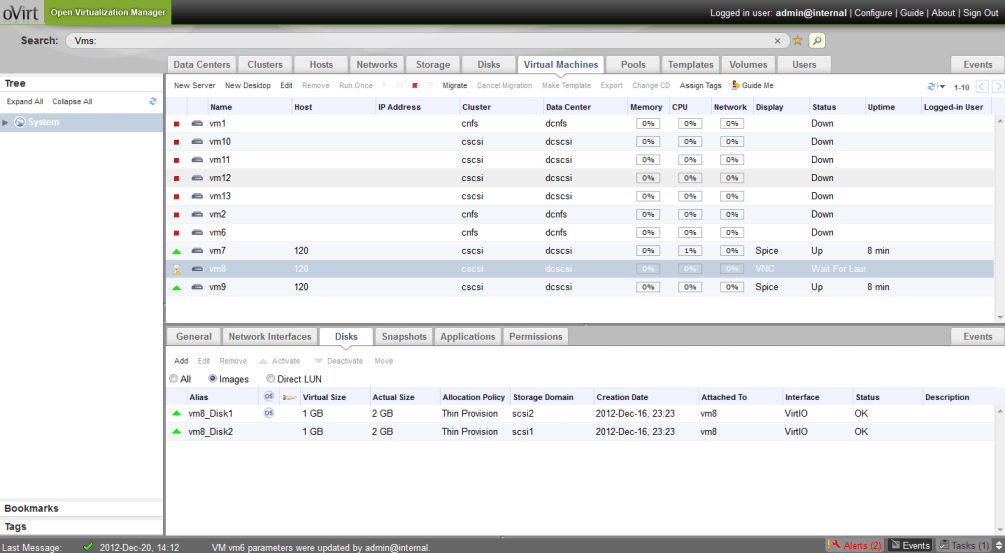
\includegraphics[scale=0.45]{ovirt.png}
\caption{oVirt}
\end{figure}

oVirt architecture consists of three main components:
\begin{enumerate}
\item oVirt Engine: Centralized virtualization management engine with graphical administration console and programming interfaces. It is a JBoss-based Java application which runs as a web service. With oVirt Engine we can deploy, monitor, move, stop and create VM images, configure storage and network, etc. oVirt Engine provides two types of portals:
\begin{enumerate}
\item Admin Portal: provides a graphical management system for administrators to manage virtual machines, templates, desktops, storage, clusters, and datacenters.
\item User Portal: provides standard and power user access to the oVirt environment.
\item oVirt API: all platform commands via an open source, community-driven RESTful API.
\item Software Development Kit: provides an Python environment to support the development of custom software utilizing the APIs exposed by the engine.
\end{enumerate}
\item host (node) on which we can run virtual machines. We can use multiple hosts.
\item storage nodes, which hold the images and ISOs corresponding to those virtual machines. Storage nodes can use block or file storage, and can be local or remote, accessed via NFS. They are grouped into storage pools, which can ensure high availability and redundancy.
\end{enumerate}

The nodes are Linux distributions with VDSM and libvirt installed, along with some extra packages to enable virtualization of networking and other system services. The supported Linux distributions are Fedora 17 or oVirt-node. oVirt Node is an image-based, small footprint hypervisor on which we run virtual machines, it is basically a stripped-down distribution containing just enough components to allow virtualization. oVirt Node provides text-based GUI for manageability and easy installation.

\section{Disadvantages of Web Admin}
oVirt's admin portal is called Web Admin and it is web based UI application running on top of the engine. Sysadmins use it to perform advanced actions. It is powerful tool for managing oVirt environment but gaining some types of information is unpractical and unnecessarily complicated.

Here are just few examples of data administrators work with that should be easier and faster to acquire:
\begin{enumerate}
\item which hosts contain unupgraded virtual machines?
\begin{enumerate}
\item Go to 'Compute' -> 'Hosts' tab
\item Choose specific host
\item Go to subtab 'Virtual Machines' to see which VMs run on that host
\item Go to 'Compute' -> 'Virtual Machines' tab
\item Choose specific virtual machine
\item In 'General' tab see compatibility version
This has to be done for every virtual machine and every host.
\end{enumerate}
\item which storage domains does particular virtual machine use?
\begin{enumerate}
\item Go to 'Storage' -> 'Domains' tab'
\item Go to 'Virtual Machines' subtab to see which VMs run on this storage domain. Remember or write down if virtual machine we are interested in is there and than do the same for every other storage domain.
\end{enumerate}
\item which virtual machine highest pressure on the network?
\begin{enumerate}
\item Go to 'Compute' -> 'Virtual Machines' tab
\item Go to 'Network Interfaces' subtab
\item Open 'Statistics' sub-subtab. Then do this for every virtual machine and remember which was using the virtual network interface the most.
\end{enumerate}
\end{enumerate}

\section{Proposed solution}
My solution to mentioned problem is a desktop application providing all the relevant information about all entities that system administrators work with. I have collaborated with several admins to design table showing all the needed data.

\begin{figure}[H]
\centering
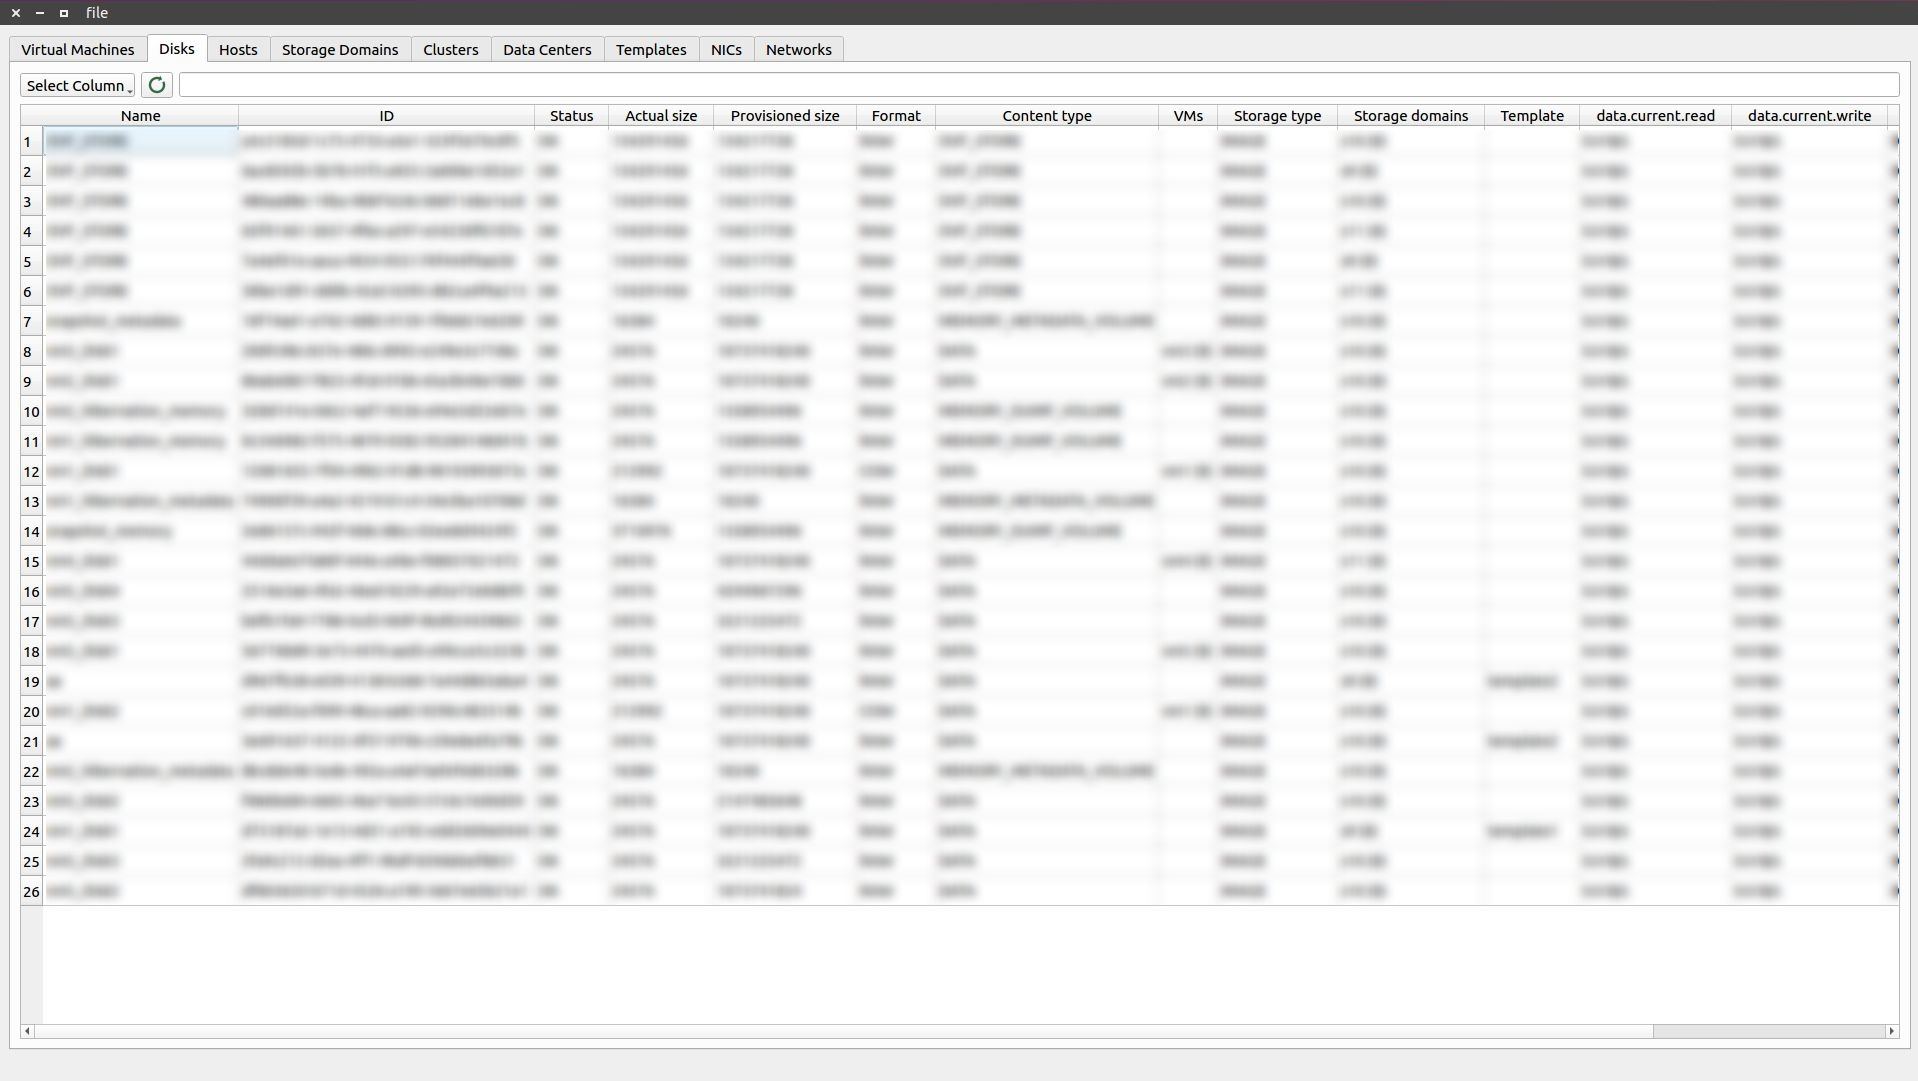
\includegraphics[scale=0.2]{tabulka.jpg}
\caption{My solution}
\end{figure}

Key features:
\begin{enumerate}
\item hiding and showing columns
\item filtering
\item sorting columns
\item export table to .csv file
\item multiple columns are linked to other columns in different tabs for easy access.
\end{enumerate}


\chapter{Implementation}
Project is implemented in programming language Python version 3.6 and PyQT5 and referential environment is operating system Fedora version 27.

\section{Back-end}
Application uses Python-SDK tool to extract all the data. The oVirt Python-SDK is an automatically generated software development kit for the oVirt engine API. This allows us to develop Python-based applications for automating a variety of complex administrative tasks in oVirt.

Application flow:
\begin{enumerate}
\item Application searches for config file.
\item After putting in login information, connection to the target virtual machine we want to inspect is established. Connection is kept during whole runtime of application. 
\item Low-level objects extract all the data needed from oVirt API.
\item High-level objects process raw data from low-level objects and form them into data structures containing refined data for all entities.
\item Tab-level objects wrap high-level objects interface and process data structures into form containing everything needed to be displayed. This includes adding row and column flags, adding filter restrictions, creating data structure for front end elements and others.
\item Tab-level objects are displayed to the user by the front-end module.
\end{enumerate}
Division of flow into hierarchy of different level modules is very important. oVirt is live and very quickly developing project. In the future, it is certain that some groups of data supported by this application will become obsolete and not needed anymore and on the other hand, there will come the demand for a new data. Whole application architecture is build with that in mind. To add or to remove column from entity, we only need to modify low-level class of given entity in trivial manner. To remove or add entirely new entity into the table, we only need to create low-level class of that entity which is simple, because if strictly follows the base low-level class. After that we create high-level class of that entity in which we only set filter restrictions, switch expressing if we want to include statistics and other attributes that cannot be set automatically. In the tab-level class we set links redirection and that is all, new entity is created, added and shown in the table. Application is very easily customizable in terms of entities it supports and data shown in each of them which will be valuable in the long run.

Supported features and functionality:
\subsubsection{Refresh}
Refresh functionality loads up to date data from API. As mentioned, connection is kept during whole run time of application. This is due to refresh functionality. If we closed connection after initial extraction of data, we would have to establish new connection every time we would want to refresh any tab which would considerably slow down process of getting new data. After losing the connection, application keeps on functioning properly but isn't able to update. Application doesn't support automatic refresh, it needs to be evoked by clicking 'refresh button'. This is due to demand of administrators I collaborated with. While investigating some failure they don't have an exclusive access to the failed virtual machine. Someone else can, for safety's sake, turn it off, restart it, delete it or something else and in that case, admins will lose the data they were working with. Automatic refresh is also very taxing and slow operation. In an environment with tens or hundreds of virtual machines, disks, etc. loading new set of data every couple of seconds would greatly slow down the application and would put unnecessary pressure on the network connection. It is also not necessary, if admins require latest data they can simply press the refresh button.

\subsubsection{Hiding and showing columns}
Entities have very many attributes and working in very large tables is impractical mainly because of horizontal scrolling. To make it easier, we can select only some currently relevant columns to be shown while other will be hidden. This configuration can be saved into 'config' file which will be loaded upon next start of the application so we don't have to always set it manually. If needed, we can still filter by hidden columns.

\subsubsection{Filtering}
Resolving filters is done by simple search engine. It supports filtering by multiple filters at the same time. Filters are in AND relationship (OR was not required by admins as there is no real use case in admin's work for it). Filters are case insensitive, and consist of these three parts: 'searched column' 'operator' 'value'. 'Searched column' is name of the column we want to filter by. 'Operator' can be '=' (equals), '>' (greater than) or '<' (less than). Columns are divided into two categories: columns containing string data (names of entities and various variables) and columns containing numeric data (values). 'Value' is value we want to filter by, it supports all Python regular expressions. Some cells contain not only one value but list of multiple values while showing only the first one and in brackets number of others. Example: one virtual machine 'vm1' uses three disks: 'Disk1', 'Disk2' and 'Disk3'. In cell is shown 'Disk1 (2)'. We can filter these kinds of cells by string regular expression or by number. If we filter them by number (disks = 2) result will be all virtual machines with 2 disks. In this manner we can similarly use '>' and '<'.  If we use filter 'disks = Disk2' result will be virtual machine 'vm1' and cell will now show 'Disk2 (2)'. Columns containing numeric data are simply filtered by value. We don;t have to include unit in the filter, engine will filter by column unit. This significantly simplifies some of admins work tasks. Here are some of supported queries useful in real-world scenarios:
\begin{enumerate}
\item A (tu pridu query)
\item B
\item C
\end{enumerate}

\subsubsection{Flags}
Application uses large set of data. To manipulate with it as little as necessary two sets of flags are used: row flags, and column flags. Filtering and hiding columns doesn't affect data, it only changes row and column flags accordingly and when printed for the user, application only prints data marked as printable by these flags. This way we only need one table of data instead of two: 'all data table' and 'currently shown data table' or even worse, constantly deleting unfit data and loading them back from the API. Not only it noticeably reduces the amount of memory needed but it increases performance as well. Flags can be stored in the 'config' file and loaded upon next start of the application so we don't have to adjust it every time and can make it more personalized.

\subsubsection{Export}
Exporting to .csv files: this is great tool for archiving data. We can choose which tables we want co save, filters and hidden columns also affect exported .csv file.

\subsubsection{Links between columns}
Some entities are in 'many to many' relationships. For example, one virtual machine can use multiple disks and similarly, one disk can contain multiple virtual machines. This relationship is hard to express in simple text table. Solution works like this: in 'Virtual machines' tab, only first disk used by any particular virtual machine is shown. In same cell there is number in brackets, this number represents number of other disks that virtual machine uses. To make it apparent, cells containing links to other tabs have light blue color. If we double click on that cell we are redirected into 'Disks' tab with only disks with virtual machine which we were redirected from shown. This way we can very simply see for example all the statistics of disks that one virtual machine is running on.

\subsubsection{Insecure mode}
Communication between application and API is not additionally secured. Added security layers are not necessary as in order to connect to the API we have to be connected into Red Hat's private virtual network (VPN) in the first place, so the communication is already secure.

\subsubsection{Ordering}
Every column can be ordered in ascending or descending order which is indicated by small arrow icon in the header of the column. Ordering and filtering use special 'custom comparison' mechanism. Table is structured in a way that cells can contain strings, integer numbers, floating point numbers, numbers with various units or without one, lists of multiple data or a special value 'None' (which is Python equivalent of 'null'). 'Custom comparison' mechanism uses operands '=', '<', '>' and can compare strings, numbers in diverse forms, lists and 'None' with each other. One limitation is that list can't be used with operators '<' and '>' which wouldn't make sense in the context of given application, they can only use '='. Here are some examples:
\begin{enumerate}
\item 'vm2' == ['vm1', 'vm2', 'vm3'] -> True (and 'vm2' will switch positions with 'vm1')
\item 'vm1' > None -> True
\item 10.2 MB < 5.245 MB -> False
\end{enumerate}

\section{Front-end}
Front end part of application uses PyQT5 module which is Python wrapper around C++ library QT5. Main focus is on simplicity and clearness of the user interface. In the spotlight is the most important part of the whole application - the table of data. Whole idea of the application is to be an effective and well functioning working tool for system administrators, so main goal is to make it minimalistic and intuitive.

Every entity is displayed in separate tab which includes drop-down menu of checkboxes for showing/hiding columns, refresh button, line edit for entering filters and table of data. In table, every virtual machine, disk, etc. printed into row and its data are in columns.


\chapter{Evaluation}



%=========================================================================
